\chapter{TMTO-Attack}
\label{ch:tmto}

To get an overview of why time-memory trade-offs were introduced, we
can first look at the two extremes exhaustive search (brute-force
attack) and a pre-computed table consisting the encryption with every
possible key. We consider a cryptographic function with the keysize
\textbf{N}. If a cryptographic function were to be attacked with these
methods, we can see it as follows
\begin{itemize}
\item The exhaustive search will, in worst case, try all $2^{N}$
  possible key combinations to try and crack the encryption. This
  requires the highest computational cost but the memory required to
  perform the attack is negligible.
\item The pre-computed table consisting of encryptions with $2^{N}$
  different keys. Only a single lookup is required when the attack is
  performed, but huge amounts of memory is required for storing the
  table. The pre-computation of the table is done only one time. 
\end{itemize}
The time-memory trade-off was introduced to improve upon these
methods and essentially combine them. In a time-memory trade-off
attack we will be able to trade memory usage at the cost of time
performing the attack and vice-versa. In this chapter we will go over
the theory of three common TMTO-attacks, namely Hellman Tables, DP
Tables and Rainbow Tables.
\section{Hellman Tables}
\label{sec:hmtheory}
Hellman trade-off is the first iteration of time-memory trade-offs. It
was first explained in the paper [Hellman - cite needed].
The idea is similar to a naive table lookup where all possible keys $K$ have been encrypted with the plaintext $P$.
Instead of storing all the key/ciphertext pairs, as done in the naive
table lookup, all pairs are sorted into several chains. In these
chains only the start point and the end point. This way memory is
saved but time is increased for finding a key $K$.

\subsection{Precomputation phase} %
Like any other TMTO-attack the table itself is generated in the
pre-computational phase.Each table is fixed for a single
plaintext. The plaintext is encrypted with the selected encryption
function $E$ and a key is a arbitrarily selected from all possible \textbf{N}
keys. This results in a ciphertext $C$ which is in turn used as the
next key for the next encryption of the plaintext. A reduction
function is applied to $C$ which has the purpose to reduce the bit
length of $C$ and re-randomize the output.


The Hellman trade-off has 3 main parameters $m$, $t$ and $l$. These will
decide the size of the table that will be generated.

$m$ is the amount of rows, $t$ is the columns, and $l$ is the amount
of tables generated.
Certain requirements that needs to hold, $m\cdot t\cdot t$ must not
neither be much larger than \textbf{N} nor much smaller. We use a
Matrix stopping constant $H_{msc}$ to hold the difference between
\textbf{N} and $m\cdot t\cdot t$. It can therefore not be very large
nor very close to zero.


add om reduction function

By selecting the parameters the table can be generated. This is done
by selecting m random starting points,
$sp^{k}_1,sp^{k}_2,...,sp^{k}_m$. Each starting point is then used as
the start of their chain and with recursion the chain links are
computed by $ x^{k}_{i,j}=F_k( x^{k}_{i,j-1})$ for $0<j<=t$. When the
end point is reached it is stored as a pair with the start point
$\{(sp^{k}_{i}, ep^{k}_{i})\}^{m}_{i=1}\}$.

The Hellman table/matrix is usually visualized as seen in figure \ref{fig:hellmax}.
\begin{figure}[th]
  \caption{from Making better tmto paper}
  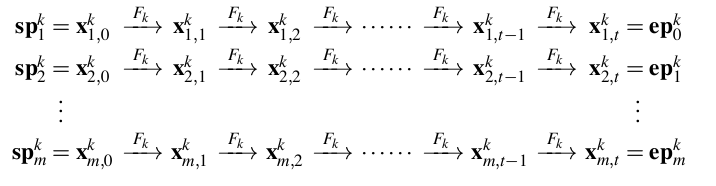
\includegraphics[width=\textwidth]{figures/HellmanMatrix.png}
  \centering
  \label{fig:hellmax}
\end{figure}

Here the starting points are $sp$ they are equal to $x$ which is the first element of the chain. It is then encrypted with the current encryption scheme and the reduction function is applied. This is done $t$ times and then $e_t$ is the endpoint.

\begin{figure}[th]
  \centering
  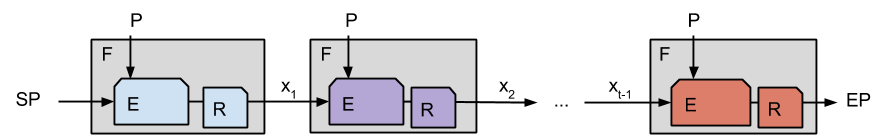
\includegraphics[width=\textwidth]{figures/HellSchema.png}
  \caption{Hellman schema}
  \label{fig:hellSchema}
\end{figure}

Each row/chain from \ref{hellmax} is built the way shown in \ref{fig:hellSchema}. When a table is generated it should contain $m$ tuples of (SP,EP) and every chain should contain $t+1$ keys which results in $m\cdot(t+1)$ keys. This should mean that our tables coverage should be m x t, this is not always the case due to merges.

\subsubsection{Merges}
Merges occur when in some point of the generation of two chains, they have the same intermediate point/chain link which causes a collision and  forces the chains merge. This is usually caused by the reduction function, if the reduction function reduces the bit-size of the ciphertext. Say we have ciphertext1 12345678 and ciphertext2 12345679 each of them are 32 bits but as our encryption only takes 28 bits then applying the reduction function to this would cause a merge since the reduction function would remove the last 4 bit. If this was the case the chains would now have merged and all the following intermediate points(chains links) will be the same. This affects the overall coverage of the table, if the merge happens 10 steps into the chain the coverage will have $10 - t$ less keys as the rest of the two chains are duplicates.
\\
\begin{figure}[th]
  \centering
  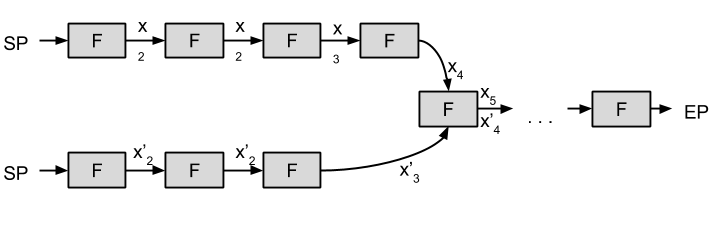
\includegraphics[width=\textwidth]{figures/Merge.png}
  \caption{Hellman schema}
  \label{fig:hellSchema}
\end{figure}
\subsubsection{Loops}
Loops occur when a intermediate point(chain link) points back to a previously reached chain link. This will also result in ad decline of the table coverage.

\begin{figure}[th]
  \centering
  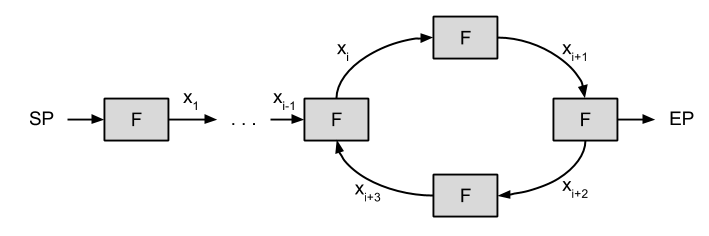
\includegraphics[width=\textwidth]{figures/Loop.png}
  \caption{Hellman schema}
  \label{fig:hellSchema}
\end{figure}

A loop will loop around in the same chain links until it reaches t.

\subsubsection{Multiple Tables}
In Hellman as m and t increases it will reach a point where the coverage will not increase due to merges and loops. This has been calculated to be somewhere near $N^{\frac{2}{3}}$ for single tables \cite{176}. A clever way to increase the success rate and coverage rate for the Hellman trade-off is by adding multiple tables.

\subsection{Online phase}
Once a table is generated and we have a matching text ciphertext pair $(y=F(x))$ the online phase can commence.\\
The given ciphertext is used as the key for the encryption and we compute a single chain. This is done for $1<k<l$ the same way as shown in \ref{fig:hellSchema} each link computed is matched with the computed Hellman table. If it reaches to the last chain link and a match is not found the algorithm will report failure.\\

Whenever a match is found the corresponding SP is returned. The chain is now partially regenerated to obtain $X_{tmp}=x^k_{i,t-j}=F^{t-j}_k(sp^k_i)$. Which should be the key the text was encrypted with:
\begin{equation}
    F^j_k(x_{tmp})=F^j_k(F^(t-j)_k(sp^k_i))=ep^k_i=y^k_j=F^{j-1}_k(y_1)=F^j_k(x)
\end{equation}
\subsubsection{False Alarms}

False alarms happen when in the online phase a match is found, but the
chain did not contain a valid key. This can happen when a chain merges
then two different chains point to the same end point.
The upper bound for false alarms in a table is $\frac{H_{msc}}{2}$


\subsection{Analysis}
This section will address the success probability, cost of resolving alarms, trade-off curve, memory usage, pre-computational time and online time.

\subsubsection*{Success probability}
The success probability of the table is found by calculating how many keys that are covered in our table. Increasing the size of the table will increase the probability that the key is in it. The amount of keys that are covered depends on the amount of start points and the size of each chain. The success ratio of a single table can be calculated the following way:\\
Lower bound from hellman paper\cite{176}
$\frac{|HM|}{N}>=\frac{1}{N}\sum^{t}_{j=1}\sum^{m}_{i=1}(1-\frac{it}{N})^{j} $
When the all the tables are processed and assuming the reduction functions provide independent results the success probability becomes:
\[1-(1-\frac{|HM|}{N})^l\approx 1- exp(-\frac{l|HM|}{N})\]
Since the count of duplicates is maintained by the matrix stopping rule, the size of the table is :$|HM|\approx mt$.
\subsubsection{Cost of resolving alarms}
The cost of resolving alarms are the following:
\begin{equation}
\text{(cost of resolving alarms for all tables)}>=\frac{H_{msc}}{6}lt
\end{equation}
proof found in \cite{176}
\begin{equation}
\text{(expected cost of resolving alarms)}=\frac{H_{msc}}{6}t
\end{equation}
proof found in \cite{176}
\subsubsection{Trade-off curve}
The trade-off curve can be found by applying the matrix stopping rule to M and T.
\begin{equation}
TM^2\approx N^2
\end{equation}
$T=t \cdot l$ and $M=m\cdot l$
Once the table has been generated it will use M memory and the online phase will take T time.

TODO More on trade-off curves

\subsubsection{Memory Usage}
Storing the table of a TMTO attack such as the Hellman trade-off takes a lot of space. Therefore it is one of the aspects of the time memory trade-off to lower the memory cost to a manageable size. The Hellman trade-off stores a tuple of a start point and a end point this can be described as $m\cdot mem$ where mem is the bit size of the  tuple stored. When several tables are used it is multiplied to the previous equation which gives:
\begin{equation}
M=m\cdot l \cdot mem
\end{equation}
where $l$ is amount of tables.
\subsubsection{Precomputational time}
Time spent on generating the tables are also a factor of the trade-off
curve, the shorter the chains the less time it takes to generate a table. There are m different start points and each of them has t chains, this means that we will use $t\cdot m$ encryptions per table. If $l$ tables are generated the formula for the Time the pre-computation takes is:
\begin{equation}
  Time=m\cdot t\cdot l
\end{equation}
Time is the amount of encryptions that will take place in the generation of the table. Therefore the real world time is Time divided by the amount of encryptions can be done pr second.

\subsubsection{Online time}
Online time is the time it takes to find a key in the worst case scenario. When searching for a key the worst case scenario is when it takes t applications of F, that is to search through the entire table. If the tradeoff consists of more than one table it is again multiplied by the amount of tables $l$.
\begin{equation}
  Time=t\cdot l
\end{equation}
The online phase is also multiplied by the time it takes one encryption or divided by the amount of encryptions per second. A major problem in the online phase of the  Hellman tradeoff is the amount of lookups needed. Even if it is possible to compute a million encryptions per second we need the capacity to access our table a million times pr second. And as our table will be stored on the harddrive it will be impossibru.



\section{Distinguished Points}
\label{sec:dptheory}

The distinguished points - trade-off was first described by Rivest in
the paper [ref] and was further analysed in \cite{DP}. It is a simple modification of the Hellman tradeoff
where one does not have chains of the same size. Instead when a
distinguished point is reached the chain does not continue. The way we distinguish a point is by some property(hence property) (eg. the first 16 bits are zero \code{dp=00001234, dp!=12345678}).Utilizing this, the amount of table lookups in the DP-trade-off is lowered dramatically, since a lookup only happens when a point that matches the property is found.
\subsection{Pre-computational phase}
The online phase of the DP-trade-off is very similar to the Hellman method.
\subsubsection{Parameters}
There are several parameters that decide the size and the coverage of
the DP-tradeoff. M is the amount of rows, t is the chain length  and l is the amount of tables.
To prevent chains from growing uncontrollably $t_{max}$ is used. This is the max size a chain can get before it is aborted and the chain discarded.
Like the Hellman tradeoff the table must satisfy the
given matrix stopping rule $mt^2\approx N$ again the difference between
mt and N should not be too large or to close to zero. Again a
matrixstopping constant is used to hold the difference $mt^2\approx
D_{msc}N$. Reduction functions are selected.... add more. The dp property is given by a bitmask with length $dp_l$.
Once the Parameters have been selected the algorithm can start. $F(SP)=C_1$ is computed and the reduction function is applied which gives the first chain link.$C_1$ is compared to the Dp property, if it is a positive match $C_1$ is an EP this is stored with the SP and the chain length $t_{DP}$. If $C_1$ does not match up with the dp property $F(C_1)=C_2$ is computed and the result compared to the dp property this is done untill an EP is found or the chain length reaches $t_{max}$
\begin{figure}[th]
  DP schema
  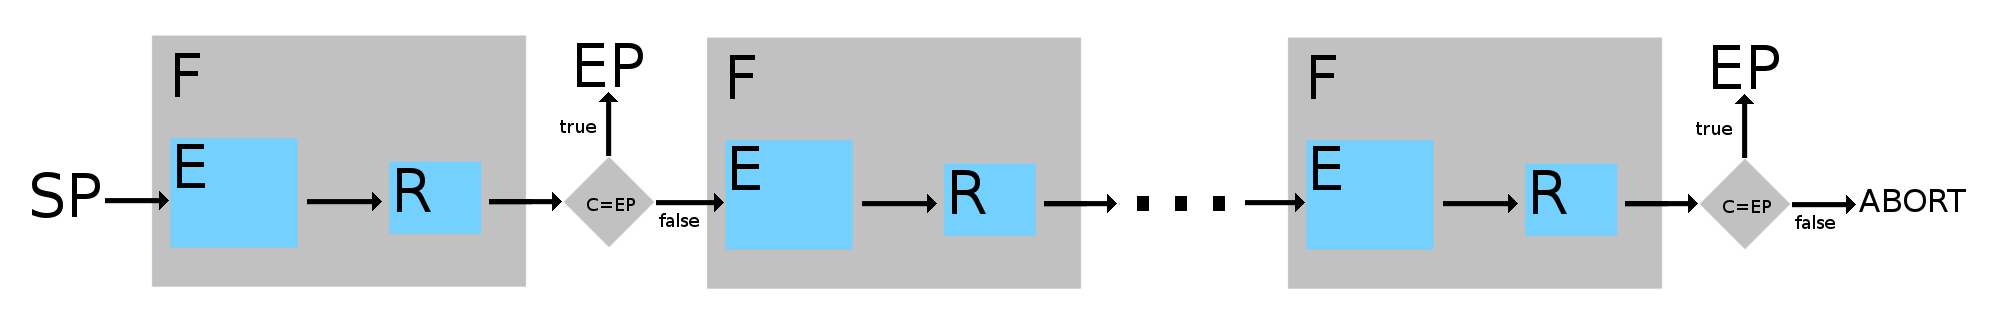
\includegraphics[width=\textwidth]{figures/DPSchema.png}
  \centering
\end{figure}
\subsection{Online phase}
The online phase for the DP-trade-off is also similar to the Hellman-tradeoff online phase. The major difference is that all EP in the computed table are distinguished points therefore instead of checking all chain links that the given ciphertext gives we only check it when a DP is reached. F is applied to C until a DP is reached or it has been applied $t_{max}-1$ times. If it reaches $t_{max}-1$ the key is not covered in the table but if it is reached we check the table for the distinguished point/EP when found we regenerate the chain from the stored SP, Just like in the Hellman tradeoff. When resolving false alarms we we either have to regenerate the entire chain untill the EP is reached. This can be prevented by storing the size of each chain in the table, this wil in turn cause the table size to increase.

\subsection{Analysis}
\subsubsection{DP Property}
The property influences the success rate, coverage, precomputation and online time. This means that the property cannot be selected arbitrarily and needs consideration. If the property requirenment is too easily met the length of each chain will decrease, which will lead to less coverage since less unique keys will be generated. If it is too hard to meet the chains will become larger but there will be less chains since some will be discarded if a point is not found. Which leads to lower coverage and a longer precomputation time. As stated the length of the dp property matters and influences the coverage and thereby the success rate of a table and can therefore neither be too large or too short. Too long chains are stored to rarely and too short chains do not consist of enough unique chain links.

The property also influences the amount of table accesses. In the online phase a chain is generated until i reaches a chain link where the property is met. The probability of finding a match is the following:
\begin{equation}
t(1-e^{-\hat{t}/t})
\end{equation}

\subsubsection{Success Ratio}
The success ratio for the DP trade-off is given by
\begin{equation}
  D_{ps}=1-e^{-D_{cr}D_{pc}}
\end{equation}
Where $D_{cr}$ is the coverage rate and $D_{pc}$ the pre-computational coefficient. Which are found by:
\begin{equation}
  D_{pc}=\frac{mtl}{N}
\end{equation}
\begin{equation}
  D_{cr}=\frac{2}{\sqrt{1+2D_{msc}}+1}
\end{equation}
When $\hat{t}$ is sufficiently large. This is when almost all chains become distinguished points. For $\hat{t}$ to be sufficiently large it should be larger than $t$ but the approximation $(1-\frac{1}{t})^{\hat{t}}\approx e^{-\hat{t}/t}$ should still remain valid.
\subsubsection{Memory Usage}
This will only cover for when $\hat{t}$ is sufficiently large.
The memory usage of the distinguished points depends on the generated table. It depends on the amount of start points, m and the bitwise size of the tuple of (SP, EP) mem and the amounts of tables generated $l$.

\begin{equation}
  M=m\cdot l \cdot mem
\end{equation}

\subsubsection{Precomputation Time}
This will only cover for when $\hat{t}$ is sufficiently large.
Due to the fact that the DP-tradeoff has no fixed chain length each chain takes an individual amount of time when constructed. And it is not allways that the chain is stored, in this case $t_{max}-1$ applications of F has been done for nothing.

\begin{equation}
  insert formula
\end{equation}

\subsubsection{Online Time}
This will only cover for when $\hat{t}$ is sufficiently large.
The online phase for distinguished points is similar to the Hellman
online phase. The length of the initial online chain computed is the
average of the length of chains in the tables L. The online time can
then be described as
\begin{equation}
  Time=L\cdot l
\end{equation}
The amount of table accesses is where the Distinguished points method really shines since in the worst case it will only do one access per table, and best case only one lookup once a point where the dp property holds has been found.

\section{Rainbow Tables}
\label{sec:raintheory}

The last type of dictionary attack we will explore, is the rainbow
attack. The rainbow attack was introduced to improve on the previous
attacks by eliminating the problem of merging chains. In a rainbow
attack the only way a chain can merge, is when a collision happens in
the same row of two pre-computational chains. As the rainbow attack uses different
reduction functions for each row of the chain, collisions happening
any other place will simply continue with different reduction
functions.

Because of this property rainbow tables will also be loop free. This
will save a lot of work compared to the two other discussed attacks.

For the rainbow attack, we will consider tables with $m$ entries build
from $t$-long pre-computational chains. The parameters $m$ and $t$
will be set such that an attack on a cryptographic
function with key size \textbf{N}, will satisfy the matrix
stopping rule $m \cdot t \approx \textbf{N}$. A matrix stopping $R_{msc}$
constant is introduced which will fulfill $m\cdot t = R_{msc} \cdot
\textbf{N}$. Another big difference between the rainbow attack and the
other discussed attacks is the small number of tables $l$, often only
one large table. As for our calculations we will mostly be looking at
rainbow attacks with only one table if nothing else is stated.

\subsection{Pre-computation Phase}

A Rainbow table is built with $m$ entries of end points, where each endpoint
$ep$ in the table is computed by a $t$ long pre-computational chain.

Each endpoint of a row is computed from a chosen/randomly chosen
start point $sp$. From the start point $sp$ the pre-computational chain,
which generates our endpoint, is computed.

For Rainbow tables, the main difference compared to the other
discussed TMTO-attacks is the reduction function. Rainbow attacks
uses $t$ different reduction functions $R_1,R_2..R_t$ to compute a pre-computation
chain of length $t$.

See \ref{fig:rainbowchain} for the structure of an $i$-th
pre-computational chain of a rainbow table.

\begin{figure}[H]
  \centering
  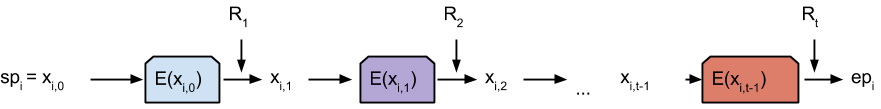
\includegraphics[scale=0.4]{figures/rainbowchain.png}
  \caption{Rainbow Chain - shows weirdly in report Fix?}
  \label{fig:rainbowchain}
\end{figure}

A full rainbow table consists of $m$ iterations of the rainbow chains
with $m$ different starting points.

If no other means of storage optimization is done each chains
starting point and ending point is stored in the rainbow table.

The pre-computation phase of a rainbow attack requires
$R_{msc} \cdot \textbf{N} \cdot l$ calls to the cryptographic function the attack targets.

\subsection{Online phase}
\label{sec:onlinerb}

The online phase of the rainbow attack differs from the other
discussed TMTO attacks, as $t$ reduction functions are used to
generate the table. To look up a key in the rainbow table one has to
compute the online chain for an input $c$. The first element of
the online chain is computed by $R_t(c)$ and looked for in the
table. If no match is found the next element $R_t(f(R_{t-1}(c)))$ is
computed and checked for a match. If nothing is found then $R_t(f(R_{t-1}(f(R_{t-2}(c)))))$
and so on. If an endpoint is found, the chain is reconstructed from the corresponding start
point. If the key is not found in the recounstructed chain it will count
as a false alarm. If the key is found the attack was a
success. This type of table lookup will leave us with at most
$\frac{t(t - 1)}{2}$ calculations of the cryptographic function and
$t$ lookups in the the table.
\subsection{Analysis}

\subsubsection{Success rate}

The success rate of a rainbow attack depends the amount of table used
and the rainbow matrix stopping constant. From \cite[Proposition
29]{176} the following describes the succes probability of a rainbow attack
\[R_{ps} = 1 - \left( \frac{2}{2+R_{msc}} \right)^{2l}\]

\subsubsection{Memory usage}

If a rainbow attack is implemented storing both start and end point,
we can expect the total storage to be 
\[M = 2 * m * bitsize\]
Optimizations can be done to the memory and result in saving
space. 




%%% Local Variables:
%%% mode: latex
%%% TeX-master: "Thesis"
%%% End:
